\subsection{ทดสอบประสิทธิภาพการทำงานของโมเดลปัญญาประดิษฐ์ Resnet50 ที่ถูกสร้างด้วยชุดข้อมูลของ AVA โดยใช้ชุดข้อมูลของ AVA ในการทดสอบและเทียบผลลัพธ์กับแหล่งอ้างอิง ได้ผลการทดลองดังตารางต่อไปนี้}
\begin{table}[!ht]
	\centering
	\begin{tabular}{|c|c|c|}
			\hline
			{}&{ความเร็วต่อรูปภาพ(มิลลิวินาที)}&{ความแม่นยำ (PASCAL mAP)}			\\
			\hline
			แหล่งอ้างอิง	 					& 93.00		& 0.110				\\
			ผลการทดสอบของผู้วิจัย				& 85.35  	& 0.068				\\
			\hline
	\end{tabular}
\caption{ผลการทดสอบความแม่นยำของโมเดลปัญญาประดิษฐ์เทียบผลลัพธ์กับแหล่งอ้างอิง}
\label{tab: Compare PASCAL mAP with source}
\end{table}
ความเร็วของต่อรูปภาพทางผู้วิจัยได้ใช้กราฟิกการ์ด GTX 2080 Ti ในการทดสอบซึ่งจะให้ความเร็วอยู่ที่ 85.35 มิลลิวินาที/ภาพ ซึ่งทางแหล่งอ้างอิงนั้นใช้กราฟิกการ์ด Nvidia GeForce GTX TITAN X 
ในส่วนของค่าความแม่นยำที่ไม่เท่ากัน คาดว่าจะเป็นเพราะการประมวลผลของกราฟิกการ์ดของรุ่นที่ต่างกันและสเปคของเครื่องคอมพิวเตอร์จึงทำให้ค่า mAP ที่ออกมาไม่เท่ากัน

\subsection{ทดสอบประสิทธิภาพการทำงานของโมเดลปัญญาประดิษฐ์ Resnet50 ที่เคยถูกสร้างด้วยชุดข้อมูลของ AVA และใช้ชุดข้อมูลที่ผู้วิจัยสร้างขึ้นในการทดสอบและเทียบผลลัพธ์กับแหล่งอ้างอิง}
\begin{table}[!ht]
	\centering
	\begin{tabular}{|c|c|c|}
			\hline
			{}&{ความเร็วต่อรูปภาพ(มิลลิวินาที)}&{ความแม่นยำ (PASCAL mAP)}			\\
			\hline
			แหล่งอ้างอิง	 					& 93.00			& 0.110			\\
			ผลการทดสอบของผู้วิจัย				& 63.11			& 0.152			\\
			\hline
	\end{tabular}
\caption{ผลการทดสอบความแม่นยำของโมเดลปัญญาประดิษฐ์ เมื่อใช้กับชุดข้อมูลที่ผู้วิจัยสร้างขึ้น}
\label{tab: Compare PASCAL mAP with dataset created by the researcher}
\end{table}
ความเร็วของต่อรูปภาพทางผู้วิจัยได้ใช้กราฟิกการ์ด Tesla V100-SXM2 ในการทดสอบซึ่งจะให้ความเร็วอยู่ที่ 63.11 มิลลิวินาที/ภาพ ซึ่งทางแหล่งอ้างอิงนั้นใช้กราฟิกการ์ด Nvidia GeForce GTX TITAN X ซึ่งการนำโมเดลปัญญาประดิษฐ์ AVA มาใช้ในการทดสอบกับชุดข้อมูลทดสอบที่ทางผู้วิจัยสร้างขึ้น ซึ่งผลลัพธ์ที่ได้ออกมานั้นสูงขึ้นหากเทียบการทดลองจากแหล่งอ้างอิง ทำให้การตั้งสมมติฐานที่ตั้งไว้ตอนแรกนั้นไม่ถูกต้อง ในส่วนที่ชุดข้อมูลที่ทางผู้วิจัยได้สร้างขึ้นจะมีการตัดหมวดหมู่ที่ไม่มีในชุดข้อมูลของ AVA ออกไป ดังนั้นจึงทำให้ผู้วิจัยสรุปได้ว่าการนำโมเดลปัญญาประดิษฐ์ของ AVA มาใช้กับชุดข้อมูลที่มีหมวดหมู่ไม่ครบก็สามารถทำงานได้มีประสิทธิภาพสูงกว่าแหล่งอ้างอิง
\clearpage
\subsection{ทดสอบประสิทธิภาพการทำงานของโมเดลปัญญาประดิษฐ์ Resnet50 ที่ถูกสร้างด้วยชุดข้อมูลที่ผู้วิจัยสร้างขึ้น และใช้ชุดข้อมูลที่ผู้วิจัยสร้างขึ้นในการทดสอบและเทียบผลลัพธ์การทดสอบก่อนหน้า}
ในส่วนนี้จะเป็นการทดสอบโดยใช้โครงสร้างโมเดลปัญญาประดิษฐ์เป็น ResNet50 โดยจะมีการใช้ชุดข้อมูลที่ผู้วิจัยสร้างขึ้นซึ่งเป็นชุดข้อมูลทดสอบเดียวกับที่ทางผู้วิจัยใช้ในการทดสอบโมเดลปัญญาประดิษฐ์ AVA มาใช้ในการทำสอบครั้งนี้ด้วย โดยชุดข้อมูลที่นำมาใช้สำหรับการสร้างโมเดลปัญญาประดิษฐ์จะมีอยู่ 2 ชุดข้อมูล ซึ่งได้แก่ goggle dataset v1 และ goggle dataset v2 ชุดข้อมูลทั้งสองอันนี้จะแตกต่างกันตรงที่ goggle dataset v2 นั้นเป็นชุดข้อมูลเกิดจากการที่ทางผู้วิจัยได้เข้าไปลบในส่วนที่มีการกำกับข้อมูลภาพผิดและมีการสุ่มตัวอย่างของข้อมูลออกมาเพื่อลดโอกาสที่จะเกิด overfitting ของข้อมูล โดยจำนวนชุดข้อมูลของ goggle dataset v1 ที่ใช้สำหรับการสร้างโมเดลจะมี 213,061 ภาพ และในส่วนของ goggle dataset v2 จะมีจำนวนชุดข้อมูล 120,177 ภาพ และมีการตั้งค่าตัวแปรต่าง ๆ ที่ใช้สำหรับการสร้างโมเดลปัญญาประดิษฐ์ดังนี้
\begin{enumerate}
	\item ขนาดของรูปภาพ : 224x224
	\item Pooling : Average pooling
	\item Activation function : Softmax
	\item Epoch : 50
	\item Batch size : 16
	\item Optimize : Momentum
	\begin{enumerate}
		\item Learning rate : 0.001
		\item Momentum : 0.9
	\end{enumerate}
\end{enumerate}
\subsubsection{การทดสอบสร้างโมเดลปัญญาประดิษฐ์ ResNet50 ด้วยชุดข้อมูล goggle dataset v1 และ goggle dataset v2}
\begin{table}[!ht]
	\centering
	\begin{tabular}{|c|c|c|}
			\hline
			{ชุดข้อมูล}&{ความเร็วต่อรูปภาพ(มิลลิวินาที)}&{ความแม่นยำ (PASCAL mAP)}			\\
			\hline
			goggle dataset v1 ResNet50			& 2.78			& 0.279				\\
			goggle dataset v2 ResNet50			& 2.52			& 0.294				\\
			\hline
	\end{tabular}
\caption{ผลการทดสอบความแม่นยำของโมเดลปัญญาประดิษฐ์ที่ผู้วิจัยสร้างขึ้น ใช้กับชุดข้อมูลที่ผู้วิจัยสร้างขึ้น}
\label{tab: Test PASCAL mAP of dataset created by the researcher}
\end{table}
จากตาราง \ref{tab: Test PASCAL mAP of dataset created by the researcher} การทดลองจะเป็นได้ว่าความเร็วของต่อรูปภาพทางผู้วิจัยได้ใช้กราฟิกการ์ด Tesla V100-SXM2 แต่ความเร็วนั้นเร็วกว่าตอนที่ทดสอบด้วยโมเดลปัญญาประดิษฐ์ AVA เป็นอย่างมาก เนื่องจากโมเดลปัญญาประดิษฐ์ของ AVA นั้นจะมีการทำในส่วนของการหากรอบสี่เหลี่ยมรอบตัวมนุษย์ด้วย ในขณะที่โมเดลปัญญาประดิษฐ์ของผู้วิจัยนั้นจะไม่มีการหากรอบสี่เหลี่ยมรอบตัวมนุษย์ เพราะจะมีการนำโมเดลปัญญาประดิษฐ์ของ YOLO-v3 spp มาหากรอบสี่เหลี่ยมรอบตัวมนุษย์ตั้งแต่แรกแล้ว ในส่วนของค่า mAP ที่ได้ออกมานั้น goggle dataset v2 มีค่า mAP มากกว่า แต่มีความแตกต่างกันไม่มาก อาจจะเป็นไปได้ว่าเพราะจำนวนข้อมูลที่น้อยกว่า goggle dataset v1 ดังนั้นทางผู้วิจัยจึงได้เลือก goggle dataset v2 มาใช้กับการทดลองครั้งต่อไป
\clearpage
\subsubsection{การทดสอบสร้างโมเดลปัญญาประดิษฐ์ ResNet50 ด้วยชุดข้อมูล goggle dataset v2 โดยใช้ weight ของ ImageNet}
\begin{table}[!ht]
	\centering
	\begin{tabular}{|c|c|c|}
			\hline
			{}&{ความเร็วต่อรูปภาพ(มิลลิวินาที)}&{ความแม่นยำ (PASCAL mAP)}			\\
			\hline
			ResNet50-ImageNet			& 2.51			& 0.454				\\
			\hline
	\end{tabular}
\caption{ผลการทดสอบความแม่นยำของโมเดลปัญญาประดิษฐ์ที่ผู้วิจัยสร้างขึ้นโดยใช้ weight จาก ImageNet ใช้กับชุดข้อมูลที่ผู้วิจัยสร้างขึ้น}
\label{tab: Test PASCAL mAP of dataset created by the researcher and pretrain weight imagenet}
\end{table}
จากตาราง \ref{tab: Test PASCAL mAP of dataset created by the researcher and pretrain weight imagenet} เมื่อทางผู้วิจัยได้นำ weight ของ ImageNet มาช่วยในการสร้างโมเดลทำให้ประสิทธิภาพของโมเดลที่ได้ออกมานั้นสูงขึ้นมากเมื่อเทียบกับการทดสอบโมเดลปัญญาประดิษฐ์ของผู้วิจัยก่อนหน้านี้

\subsubsection{การทดสอบสร้างโมเดลปัญญาประดิษฐ์ ResNet50-ImageNet ด้วยชุดข้อมูล goggle dataset v2 ด้วยวิธีการทำ scaling}
\begin{table}[!ht]
	\centering
	\begin{tabular}{|c|c|c|}
			\hline
			{}&{ความเร็วต่อรูปภาพ(มิลลิวินาที)}&{ความแม่นยำ (PASCAL mAP)}			\\
			\hline
			ResNet50-ImageNet	 Normalization				& 2.51			& 0.449				\\
			ResNet50-ImageNet	 Centering Featurewise		& 2.40			& 0.457				\\
			ResNet50-ImageNet	 Centering Samplewise		& 2.49			& 0.466				\\
			ResNet50-ImageNet	 Standardize Featurewise		& 2.48			& 0.407				\\
			ResNet50-ImageNet	 Standardize Samplewise		& 2.49			& 0.432				\\
			\hline
	\end{tabular}
\caption{ผลการทดสอบความแม่นยำของโมเดลปัญญาประดิษฐ์ที่ผู้วิจัยสร้างขึ้นโดยใช้ weight จาก ImageNet และการทำ scaling ใช้กับชุดข้อมูลที่ผู้วิจัยสร้างขึ้น}
\label{tab: Test PASCAL mAP of dataset created by the researcher with pretrain weight imagenet and scaling}
\end{table}

จากตาราง \ref{tab: Test PASCAL mAP of dataset created by the researcher with pretrain weight imagenet and scaling} จะเป็นการทดลอง scaling ด้วยรูปแบบต่าง ๆ โดยสาเหตุที่เลือกการใช้วิธีการทำ scaling เป็นเพราะทางผู้วิจัยได้คิดว่าข้อมูลของการกระทำในภาพนั้นมีความสัมพันธ์กัน แต่ว่าด้วยสภาพของแสงหรือมุมของกล้องที่ทำการเก็บวิดีโอนั้นอาจจะทำให้ค่าของข้อมูลภาพนั้นมีช่วงที่แตกต่างกัน จึงได้นำวิธีการ scaling มาใช้งานอย่างการทำ normalization จะเป็นทำให้ค่าในพิกเซลอยู่ในช่วง 0 ถึง 1 การทำ centering คือการลบค่าในพิกเซลด้วยค่าเฉลี่ยของพิกเซล โดยจะแบ่งออกเป็น 2 แบบได้แก่ featurewise และ samplewise โดย featurewise จะเป็นการหาค่าเฉลี่ยพิกเซลจากทุกรูปในชุดข้อมูลแล้วนำมาลบออกในแต่ละพิกเซลของรูป ส่วนของ samplewise จะไม่มีการไปยุ่งเกี่ยวกับรูปอื่น คือจะหาค่าเฉลี่ยของพิกเซลของรูปนั้น ๆ และนำค่าพิกเซลในรูปนั้น ๆ ลบออกด้วยค่าเฉลี่ย ต่อมาการทำ standardize คือการหารค่าในพิกเซลด้วยค่า standard deviation ของพิกเซลในรูป ซึ่งจะแบ่งออกเป็น 2 แบบ ได้แก่ featurewise และ samplewise เหมือนกับ centering โดย featurewise จะหาค่า standard deviation ของทุกพิกเซลในชุดข้อมูลแล้วนำมาหารในแต่ละพิกเซลของรูป ส่วนของ samplewise จะเป็นการหาค่า standard deviation ของรูปนั้น ๆ มาหารกับทุกพิกเซลในรูปนั้น ๆ จากการทำลองจะทำให้เห็นว่าโมเดลปัญญาประดิษฐ์ที่มีประสิทธิภาพสูงที่สุดคือโมเดลปัญญาประดิษฐ์ ResNet50-ImageNet	 Centering Samplewise
\clearpage
\subsubsection{การทดสอบ average preicision (AP) ของโมเดลปัญญาประดิษฐ์ ResNet50-ImageNet Centering Samplewise}
\begin{table}[!ht]
	\centering
	\begin{tabular}{|c|c|c|}
			\hline
			{Label}&{ResNet50-ImageNet Centering Samplewise}			\\
			\hline
			Play phone				& 0.824			\\
			Eat						& 0.975			\\
			Sit						& 0.215			\\
			Sleep					& 0.473			\\
			Stand					& 0.043			\\
			Walk					& 0.266			\\
			\hline
	\end{tabular}
\caption{โมเดลปัญญาประดิษฐ์ ResNet50-ImageNet	 Centering Samplewise วัดค่า average precision (AP) ของแต่ละหมวดหมู่}
\label{tab: ResNet50-ImageNet Centering Samplewise average precision}
\end{table}

\begin{figure}[!ht]
  \centering
    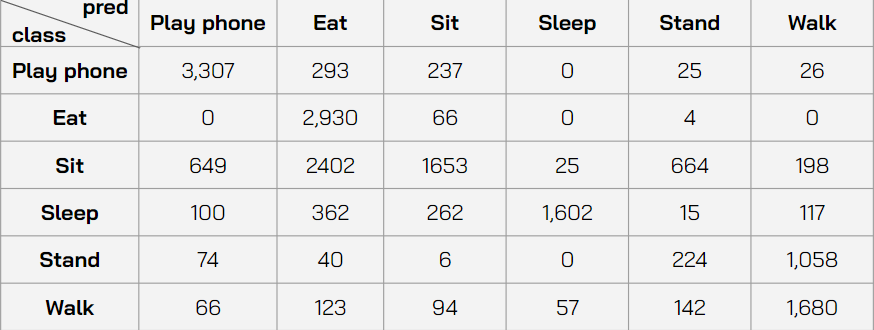
\includegraphics[scale=0.5]{chapter4/images/confusion_matrix.png}
    \caption{Confusion matrix ของโมเดลปัญญาประดิษฐ์  ResNet50-ImageNet Centering Samplewise}
    \label{fig:Confusion matrix of ResNet50-ImageNet Centering Samplewise model}
\end{figure}

จากตาราง \ref{tab: ResNet50-ImageNet Centering Samplewise average precision} และรูปภาพที่ \ref{fig:Confusion matrix of ResNet50-ImageNet Centering Samplewise model} จะเห็นได้ว่าหมวดหมู่ที่ได้ค่า average precision น้อยได้แก่หมวดหมู่ sit, stand และ walk จากหมวดหมู่ sit นั้นที่ได้ค่า  average precision น้อยนั้นเป็นเพราะว่าการกระทำนั้นใกล้เคียงกับท่าทางการกระทำของ eat และในส่วนของหมวดหมู่ stand และ walk จะเป็นเพราะว่ามีการทำนายในหมวดหมู่ของ stand ส่วนใหญ่จะทำนายออกมาเป็นหมวดหมู่ walk เพราะทั่งสองหมวดหมู่นี้มีการกระทำที่คล้ายคลึงกัน

\clearpage
\subsection{ทดสอบประสิทธิภาพการทำงานของโมเดลปัญญาประดิษฐ์ I3D สร้างด้วยชุดข้อมูลที่ผู้วิจัยสร้างขึ้น โดยใช้ชุดข้อมูลที่ผู้วิจัยสร้างขึ้นในการทดสอบ}
คุณลักษณะที่ใช้ในการสร้างโมเดลปัญญาประดิษฐ์ I3D ที่ผู้วิจัยได้พัฒนาเป็นชุดของเฟรมที่เป็นภาพสีปกติ (RGB) และชุดของเฟรมที่เป็น optical flow (OF) โดยใช้ PASCAL mAP, Top@1 และ Top@3
ในการวัดผลความแม่นยำของแต่ละโมเดล ซึ่งมีรายละเอียดและพารามิเตอร์ดังนี้
\begin{enumerate}
	\item โมเดลที่ 1
	\begin{enumerate}
		\item Learning rate: 0.001
		\item Dropout: 0.36
		\item Optimizer: Momentum
		\item Optimizer parameter:
		\begin{enumerate}
			\item Momentum: 0.8
		\end{enumerate}
	\end{enumerate}
	\item โมเดลที่ 2
	\begin{enumerate}
		\item Learning rate: 0.001
		\item Dropout: 0.36
		\item Optimizer: Adam
		\item Optimizer parameters:
		\begin{enumerate}
			\item $\beta_1$: 0.9
			\item $\beta_2$: 0.999
			\item $\epsilon$: $10^{-8}$
		\end{enumerate}
	\end{enumerate}
\end{enumerate}


\subsubsection{การทดสอบประสิทธิภาพของโมเดลปัญญาประดิษฐ์ I3D ที่ใช้ชุดข้อมูลที่เป็นแบบภาพสีปกติ}
\begin{table}[!ht]
	\centering
	\begin{tabular}{|c|c|c|c|}
			\hline
			{โมเดล}	&	{PASCAL mAP}	&	{Top@1}	&	{Top@3}\\
			\hline
			RGB โมเดลที่ 1	& 0.564	& 0.482	& 0.641	\\
			RGB โมเดลที่ 2	& 0.356	& 0.265	& 0.487	\\
			\hline
	\end{tabular}
\caption{ผลการทดสอบความแม่นยำของโมเดลปัญญาประดิษฐ์ที่ผู้วิจัยสร้างขึ้นโดยใช้ชุดข้อมูลที่ผู้วิจัยสร้างขึ้นแบบภาพสีปกติ}
\label{tab:I3D_RGB_performance}
\end{table}

\subsubsection{การทดสอบประสิทธิภาพของโมเดลปัญญาประดิษฐ์ I3D ที่ใช้ชุดข้อมูลที่เป็นแบบ optical flow}
\begin{table}[!ht]
	\centering
	\begin{tabular}{|c|c|c|c|}
			\hline
			{โมเดล}	&	{PASCAL mAP}	&	{Top@1}	&	{Top@3}\\
			\hline
			Optical flow โมเดลที่ 1	& 0.748	& 0.737	& 0.908	\\
			Optical flow โมเดลที่ 2	& 0.777	& 0.759	& 0.959	\\
			\hline
	\end{tabular}
\caption{ผลการทดสอบความแม่นยำของโมเดลปัญญาประดิษฐ์ที่ผู้วิจัยสร้างขึ้นโดยใช้ชุดข้อมูลที่ผู้วิจัยสร้างขึ้นแบบ optical flow}
\label{tab:I3D_OF_performance}
\end{table}


\subsubsection{ตารางแสดงการเปรียบเทียบค่า average precision (AP) ของทุกการกระทำของแต่ละโมเดล}
\label{sec:I3D_AP}
\begin{table}[!ht]
	\centering
	\begin{tabular}{|c|c|c|c|c|}
			\hline
			{Label} & {RGB โมเดลที่ 1} & {RGB โมเดลที่ 2} & {OF โมเดลที่ 1} & {OF โมเดลที่ 1}\\
			\hline
			Play phone  & 0.239 & 0.011 & 0.552 & 0.599	\\
			Eat			& 0.282	& 0.058	& 0.787	& 0.839	\\
			Sit		 	& 0.450 & 0.113 & 0.795 & 0.799	\\
			Sleep		& 0.800	& 0.655	& 0.704	& 0.628	\\
			Stand		& 0.865	& 0.822	& 0.731	& 0.797	\\
			Walk		& 0.748	& 0.476	& 0.921	& 1.000	\\
			\hline
	\end{tabular}
\caption{ตารางเปรียบเทียบค่า AP ของทุกการกระทำของแต่ละโมเดล}
\label{tab:I3D_RGB_OF_AP}
\end{table}
จะเห็นได้ว่าโมเดลที่ถูกสร้างจากชุดข้อมูลแบบ optical flow นั้นมีความแม่นยำสูงกว่าโมเดลที่ใช้ข้อมูลภาพสีแบบปกติในการสร้าง แต่ถ้าหากพิจารณาจากค่า average precision (AP) 
ตามตารางที่ \ref{tab:I3D_RGB_OF_AP} โมเดลที่ผ่านการสร้างด้วยชุดข้อมูลแบบภาพสีปกตินั้นจะมีประสิทธิภาพสูงเมื่อเป็นการกระทำที่แทบจะไม่มีการเคลื่อนไหวคือ นอนและยืน 
ในขณะที่โมเดลที่ผ่านการสร้างด้วยชุดข้อมูลแบบ optical flow นั้นมีความแม่นยำสูงกว่ามากในการกระทำที่มีการเคลื่อนไหว จึงสามารถกล่าวได้ว่าโมเดลแบบ optical flow 
นั้นเหมาะสำหรับใช้ในการจำแนกการกระทำที่มีการเคลื่อนไหว และโมเดลแบบภาพสีปกติเหมาะสำหรับใช้ในการจำแนกการกระทำที่แทบจะไม่มีการเคลื่อนไหว

\subsubsection{การทดสอบประสิทธิภาพของโมเดลปัญญาประดิษฐ์ I3D ที่ใช้ชุดข้อมูลทั้งสองแบบ (RGB + optical flow)}
จากผลการวิเคราะห์ในหัวข้อที่ \ref{sec:I3D_AP} ทำให้ผู้วิจัยสนใจนำโมเดลทั้งสองแบบมาใช้ร่วมกันในการจำแนกการกระทำ โดยจะใช้การรวมผลลัพธ์ความน่าจะเป็นที่ถูกคูณด้วยอัตราส่วนความน่าเชื่อถือ
หมายความว่าในการกระทำ $l$ โมเดล $M_1$ ทำนายผลออกมาว่ามีความเป็นไปได้ว่าชุดข้อมูลนี้จะเป็นการกระทำดังกล่าว $P_l^{M_1}$ 
และโมเดล $M_2$ ทำนายผลออกมาว่ามีความเป็นไปได้ว่าชุดข้อมูลนี้จะเป็นการกระทำดังกล่าว $P_l^{M_2}$ สมมติว่าให้อัตราส่วนความน่าเชื่อถือของโมเดล $M_1$ เป็น $W_1$
และของโมเดล $M_2$ เป็น $W_2$ (โดยที่ $W_1 + W_2 = 1$) ทำให้สามารถเขียนสมการความเป็นไปได้ว่าชุดข้อมูลนี้จะเป็นการกระทำ $l$ ได้ดังนี้
\begin{equation}
	P_l = \frac{W_1 P_l^{M_1} + W_2 P_l^{M_2}}{2}
\end{equation}
ซึ่งผลลัพธ์จากการทดลองเป็นดังตารางที่ \ref{tab:I3D_RGB_OF_performance} และผลลัพธ์ค่า average precision เป็นดังตารางที่ \ref{tab:I3D_RGB_OF_AP}
\begin{table}[!ht]
	\centering
	\begin{tabular}{|c|c|c|c|}
			\hline
			{โมเดล (อัตราส่วนความน่าเชื่อถือ)}	&	{PASCAL mAP}	&	{Top@1}	&	{Top@3}\\
			\hline
			RGB โมเดลที่ 1 + OF โมเดลที่ 1 (50:50)	& 0.765	& 0.740	& 0.903	\\
			RGB โมเดลที่ 1 + OF โมเดลที่ 2 (50:50)	& 0.823	& 0.806	& 0.945	\\
			RGB โมเดลที่ 2 + OF โมเดลที่ 1 (50:50)	& 0.706	& 0.679	& 0.865	\\
			RGB โมเดลที่ 2 + OF โมเดลที่ 2 (50:50)	& 0.804	& 0.780	& 0.931	\\
			\hline
	\end{tabular}
\caption{ผลการทดสอบความแม่นยำเมื่อนำโมเดลแบบภาพสีปกติ และ optical flow มาใช้ร่วมกัน}
\label{tab:I3D_RGB_OF_performance}
\end{table}
จากผลลัพธ์ในตารางที่ \ref{tab:I3D_RGB_OF_performance} จะเห็นว่าเมื่อนำโมเดลทั้งสองแบบมาใช้งานร่วมกันด้วยอัตราส่วนความน่าเชื่อถือ 50:50 ทำให้ประสิทธิภาพโดยรวมสูงขึ้น
ซึ่งหากลองพิจารณาจากประสิทธิภาพในแต่ละการกระทำ ด้วยค่า average precision จะได้ผลลัพธ์ดังตารางที่ \ref{tab:I3D_RGB_w_OF_AP} 
จากตารางจะเห็นว่าประสิทธิภาพในการจำแนกการกระทำนั้นมีความครอบคลุมมากกว่าการใช้โมเดลแบบเดียวในการทำนายผล แต่การเล่นโทรศัพท์ (play phone) ยังคงมีประสิทธิภาพที่ต่ำมาก
ทั้งนี้ผู้วิจัยได้ตรวจสอบแล้วพบว่าการทำนายที่ผิดส่วนมากจะเป็นการนั่ง (sit) ผู้วิจัยจึงคาดว่าเกิดจากการที่การเคลื่อนไหวของการเล่นโทรศัพท์นั้นมีความใกล้เคียงกับการนั่งมาก
จึงทำให้การโมเดลสามารถแยกความแตกต่างออกได้ยาก
\begin{table}[!ht]
	\centering
	\begin{tabular}{|c|c|c|c|c|}
		\hline
		{Label} & {RGB\textsubscript{1}+OF\textsubscript{1}} & {RGB\textsubscript{1}+OF\textsubscript{2}} & {RGB\textsubscript{2}+OF\textsubscript{1}} & 
		{RGB\textsubscript{2}+OF\textsubscript{2}}\\
		\hline
		Play phone  & 0.544	& 0.581	& 0.405	& 0.574	\\
		Eat			& 0.785	& 0.836	& 0.827	& 0.847	\\
		Sit		 	& 0.705	& 0.791	& 0.685	& 0.772	\\
		Sleep		& 0.852	& 0.963	& 0.825	& 0.981	\\
		Stand		& 0.883	& 0.881	& 0.840	& 0.809	\\
		Walk		& 0.824	& 0.884	& 0.653	& 0.841	\\
		\hline
	\end{tabular}
\caption{ตารางเปรียบเทียบค่า AP ของทุกการกระทำของแต่ละโมเดล}
\label{tab:I3D_RGB_w_OF_AP}
\end{table}
